\documentclass[12pt]{article}

\usepackage{amssymb,amsmath,amsfonts,bbm,bm,dcolumn,booktabs,eurosym,geometry,ulem,graphicx,color,xcolor,setspace,sectsty,comment,float,caption,subfigure,array,hyperref}
\usepackage{xurl}
\usepackage[font=bf]{caption}
\usepackage[bottom]{footmisc}

\hypersetup{
    colorlinks,
    linkcolor={black},
    citecolor={blue!35!black},
    urlcolor={blue!35!black}
}

\geometry{left=1.0in,right=1.0in,top=1.0in,bottom=1.0in}

\begin{document}
\title{Development Economics Problem Set 1}
\author{Steven VanOmmeren\thanks{A complete replication package of this project is available at \url{https://github.com/svanomm/development-econ/}.}}
\date{\today}
\maketitle

\doublespacing
\section{Introduction}
The Human Development Index (HDI) is a composite statistic of life expectancy, education, and per capita income indicators, which is used to assess the economic ``health'' of a country. HDI is calculated using three components: health, education, and income. The health component is measured by life expectancy at birth, the education component is measured by mean years of schooling and expected years of schooling, and the income component is measured by log of gross national income (GNI) per capita adjusted for purchasing power parity (PPP). For my assignment, I am interested in using the World Bank's World Development Indicators (WDI) dataset to create a proxy of HDI. Additionally, I create a ``Female HDI" that substitutes some of the indexes with female-specific ones, with the hypothesis that an HDI evaluated on women could reflect gender inequality not accounted for by the original HDI.

\section{Methodology}
My data comes from the World Bank's World Development Indicators (WDI) dataset, downloaded as a CSV file.\footnote{\url{https://datacatalog.worldbank.org/search/dataset/0037712}.} I used the \textsf{pandas} package in Python to join the data, clean it, and prepare it for analysis.\footnote{\url{https://pandas.pydata.org/}.} After joining the relevant files, I identified the variables that are relevant to calculating my HDI proxies:
\begin{itemize}
    \singlespace
    \item Life expectancy at birth, total (years),
    \item Compulsory education, duration (years),
    \item Educational attainment, at least completed primary, population 25+ years, total (\%) (cumulative),
    \item Educational attainment, at least completed lower secondary, population 25+, total (\%) (cumulative),
    \item Educational attainment, at least completed upper secondary, population 25+, total (\%) (cumulative),
    \item GNI per capita, PPP (current international \$).
\end{itemize}

I additionally included the following variables for creating the Female HDI:
\begin{itemize}
    \singlespace
    \item Life expectancy at birth, female (years),
    \item Educational attainment, at least completed primary, population 25+ years, female (\%) (cumulative),
    \item Educational attainment, at least completed lower secondary, population 25+, female (\%) (cumulative),
    \item Educational attainment, at least completed upper secondary, population 25+, female (\%) (cumulative).
\end{itemize}

My education variables are different from the UN's data. As a proxy for expected years of schooling, I use the duration of compulsory education. As a proxy for mean years of schooling, my variables report a percentage of the population that has completed a given level of education. I chose three different levels of education to capture a wide range of educational attainment for each country. While I give equal weight to each metric, the weights could be adjusted to give more importance to primary education, for example.

Lastly, I included GDP and GDP per capita, both adjusted for purchasing power parity (PPP). I also took the log of both of these variables.

In preparing my data, I found that some of these variables are missing for some countries and years. I used 2023 data when available, and otherwise used the most recently available observation for each country (from 2015 to 2022). After this imputing process, I dropped any countries that still had missing values. This left me with 171 out of the original 217 countries.\footnote{Dropping countries with missing data is a potential source of selection bias in my data. Developing countries are more likely to have missing data, so by dropping them I may be biasing my sample towards higher-income countries.} I then took a simple random sample of 100 countries for my analysis.

The HDI is calculated using indexes of the original variables. For example, the UN calculates the life expectancy index as follows:\footnote{\url{https://hdr.undp.org/sites/default/files/2025_HDR/HDR25_Technical_Notes.pdf}, at p. 3.}
$$\text{Life Expectancy Index} = \frac{\text{Life Expectancy} - 20}{85 - 20}.$$
Similarly, the expected years of schooling index is calculated as follows:
$$\text{Expected Years of Schooling Index} = \frac{\text{Expected Years of Schooling} - 0}{18 - 0}.$$

I calculated my indexes using two different methods: an ``Absolute" method and a ``Relative" method. The Absolute method uses the the minimum and maximum values as defined by the UN.\footnote{Since I do not use mean years of schooling, my proxy variables use a minimum of 0\% and maximum of 100\%.} The Relative method uses the minimum and maximum values observed in my sample of countries. The UN uses the relative method when calculating the income component of the HDI.

After averaging the education indexes, I calculated HDI using a geometric mean of the health, education, and log income indexes, following the UN's method.

I also downloaded the UN's latest HDI data to compare to my HDI proxies.\footnote{\url{https://hdr.undp.org/data-center/human-development-index\#/indicies/HDI}.} I had to perform additional cleaning to align the country names between the datasets. After joining the data, I calculated the correlation between the UN's HDI, and my metrics.

\section{Results}
Below shows the correlation matrix of my HDI proxies, the UN HDI, and GDP/log of GDP. Overall, the Female HDI proxies are almost the same as my original HDI proxies. All 4 of my HDI proxies are highly correlated with the UN HDI (around 97\%). My HDI measures have higher correlation with Log GDP than with GDP, which is expected since the HDI uses a logarithm for the income index.

\begin{table}[H]
    \footnotesize
\caption{Correlation Results}
\begin{tabular}{lcccc}
\toprule
 & HDI Relative & HDI Relative Female & HDI Absolute & HDI Absolute Female \\
\midrule
HDI Relative & 1.000 & 0.998 & 0.978 & 0.977 \\
HDI Relative Female & 0.998 & 1.000 & 0.979 & 0.980 \\
HDI Absolute & 0.978 & 0.979 & 1.000 & 0.999 \\
HDI Absolute Female & 0.977 & 0.980 & 0.999 & 1.000 \\
UN HDI & 0.976 & 0.975 & 0.974 & 0.974 \\
GDP, PPP & 0.131 & 0.126 & 0.131 & 0.125 \\
Log GDP, PPP & 0.304 & 0.286 & 0.311 & 0.294 \\
\bottomrule
\end{tabular}
\end{table}


Below are scatterplots of my HDI proxies against log of GDP PPP for my sample of 100 countries. I have colored the points based on the World Bank's income group classification, and fit regression lines through each group. The slope of each regresion line is positive and generally consistent across income groups, though high income countries almost always have higher HDI than lower income countries. This is expected because income is part of the HDI calculation.

\begin{figure}[H]
\centering
\caption{Scatterplot of HDI Absolute against Log GDP PPP}
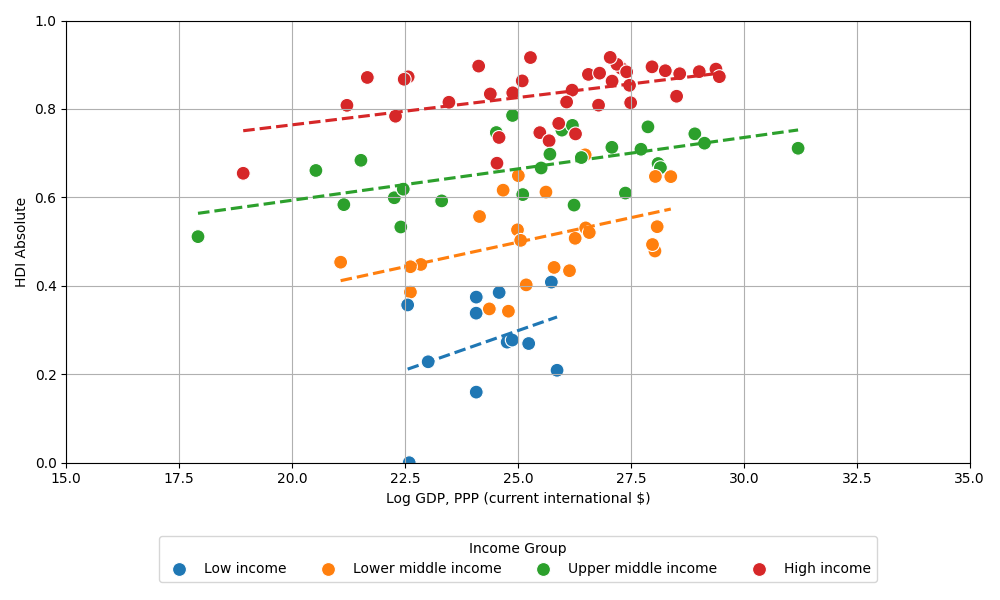
\includegraphics[width=0.8\textwidth]{./output/Scatterplot HDI Absolute.png}
\label{fig:scatter_hdi_absolute}
\end{figure}

\begin{figure}[H]
\centering
\caption{Scatterplot of HDI Relative against Log GDP PPP}
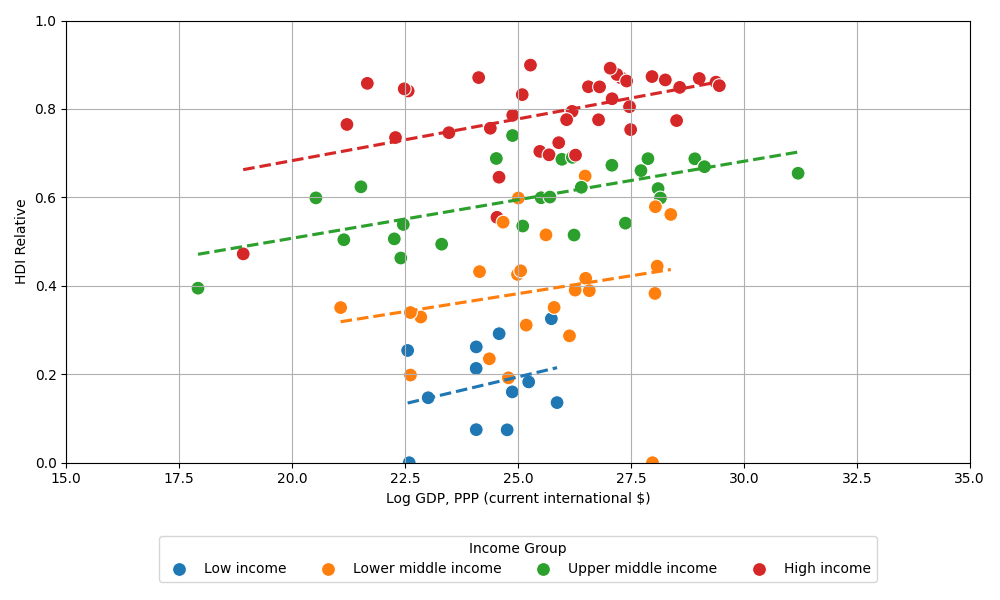
\includegraphics[width=0.8\textwidth]{./output/Scatterplot HDI Relative.png}
\label{fig:scatter_hdi_relative}
\end{figure}

\section{Discussion}
 One of the criticisms of the HDI is that it is sensitive to the maximum and minimum values used by the UN. However, comparing Figure \ref{fig:scatter_hdi_absolute} with Figure \ref{fig:scatter_hdi_relative} shows that with a sample size of 100 countries, the relative method produces similar results to the absolute method. This is also seen in my correlation matrix, where the correlations between absolute and relative measures are very high. One issue I noticed is that with the relative method, the minimum country for each component index will have an HDI of 0 because of the geometric mean formula being a product of the components. The absolute method only produces an HDI of 0 if all of the indexes are 0. We can see in Figure \ref{fig:scatter_hdi_relative} that there is an additional orange point at HDI Relative = 0.

 As discussed above, my HDI measures have higher correlation with Log GDP than with GDP. However, both correlations are relatively weak, at around 13\% for GDP and 30\% for Log GDP. There are many reasons why we could expect these results. There should be a positive correlation because, generally speaking, countries with higher GDP have more government resources to invest in health and education, improving the HDI. However, the correlations are relatively weak because GDP does not control for population, so high population countries like China have higher GDP than Australia (for example), though Australia is richer on a per-capita basis. Additionally, GDP does not consider the distribution of wealth, so countries with very high wealth inequality could have a high GDP but still have a large portion of its population in poverty.

Going into this analysis, one criticism I expected of the HDI was that it does not account for gender inequality. I expected that calculating the HDI for females only would widen the distribution of HDI scores (with Low-HDI countries having more gender inequality than high-HDI ones). However, my correlation results show that the female HDI proxies are almost identical to the original HDI proxies, indicating that any differences in gender inequality are already baked into the HDI metrics. It is also very likely that my choice of variables do not represent the full extent of gender inequality in a country, but I wanted to keep my variables in line with the HDI components.
\end{document}